\chapter{Uniswap}

\section{Overview}
Uniswap is a decentralized exchange protocol built on the Ethereum blockchain. It allows users to trade ERC-20 tokens directly from their wallets without the need for intermediaries or traditional order books. Uniswap utilizes automated market-making, where liquidity providers contribute funds to liquidity pools, earning fees on trades made in the pool. The protocol employs a mathematical formula called the constant product formula to maintain balanced token ratios in the pool. When users want to make a trade, Uniswap calculates the conversion based on the pool's token ratios and executes the trade through a smart contract.

\section{How it works}
\subsection{Automated Market Maker (AMM) Model and Liquidity Pools}
The AMM model is a system that replaces traditional order books with liquidity pools to facilitate trading between different tokens. Automated Market Makers do this with the aid of liquidity pools. They are pools of tokens contributed by liquidity providers (LPs) to facilitate trading between different tokens within the exchange. One paper describes pools as ``a smart contract that holds at least two cryptoassets and allows trading through depositing a token of one type and thereby withdrawing tokens of the other type''~\cite{schar2021decentralized}. These liquidity pools are maintained by smart contracts on Ethereum and Liquidity Providers (LPs). Liquidity providers are individuals that voluntarily contribute an equal amount of cryptocurrencies liquidity pools, for example, in a pool for trading ETH and DAI, LPs would contribute an equal value of ETH and DAI tokens. LPs are incentivised to do provide liquidity in exchange for a share of the trading fees that occur in the liquidity pool. LPs can later withdraw their shares along with the accumulated fees. On Uniswap V3, the fee is 0.3\% on Ethereum, however they can be any of 0.01\%, 0.05\%, 0.3\%, or 1\% depending on blockchain network.

\subsection{Constant Product Formula}
To maintain a balanced ratio between the tokens in the pool and price any swaps, the AMM model relies on a mathematical formula called the constant product formula ($xy = k$). As trades occur, the product of the token balances remains constant. When one token's value increases, its proportion in the pool decreases, ensuring an automatic adjustment in prices. When a trade is executed, the change in prices can be described in this formula $(x + \Delta x)(y + \Delta y) = k$. Hence, after rearranging: $\Delta y = \frac{k}{x + \Delta x} - y$. Under this model, the balance of the tokens in a liquidity pool can never be depleted as the token will get infinitely more expensive as the reserves approach 0.

\begin{figure}[!htb]
    \centering
    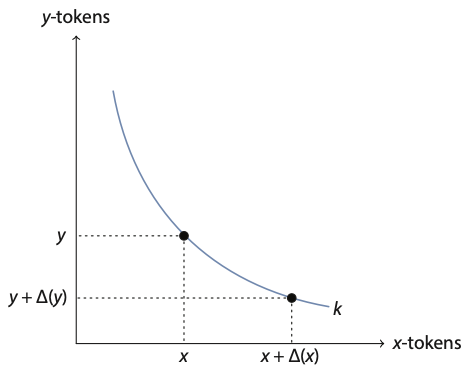
\includegraphics[width=0.5\textwidth]{background/Images/constant_product_formula.png}
    \caption{Constant Product Formula~\cite{schar2021decentralized}}
\end{figure}

\subsection{Slippage}

As seen in Figure \ref{fig:uniswap_lp}, we can see how the constant product formula is used in Uniswap. Uniswap also allow users to set slippage tolerance levels, which determine the maximum acceptable difference between the expected and executed prices. Slippage refers to the difference between the expected price of a trade and the executed price due to market volatility and liquidity conditions. Slippage happens because the constant product formula adjusts prices based on the ratio of tokens in the pool. As trades are executed, the token balances change, and the prices change accordingly. Thus, larger trades can cause more significant price impact, resulting in slippage.

\begin{figure}[!htb]
    \centering
    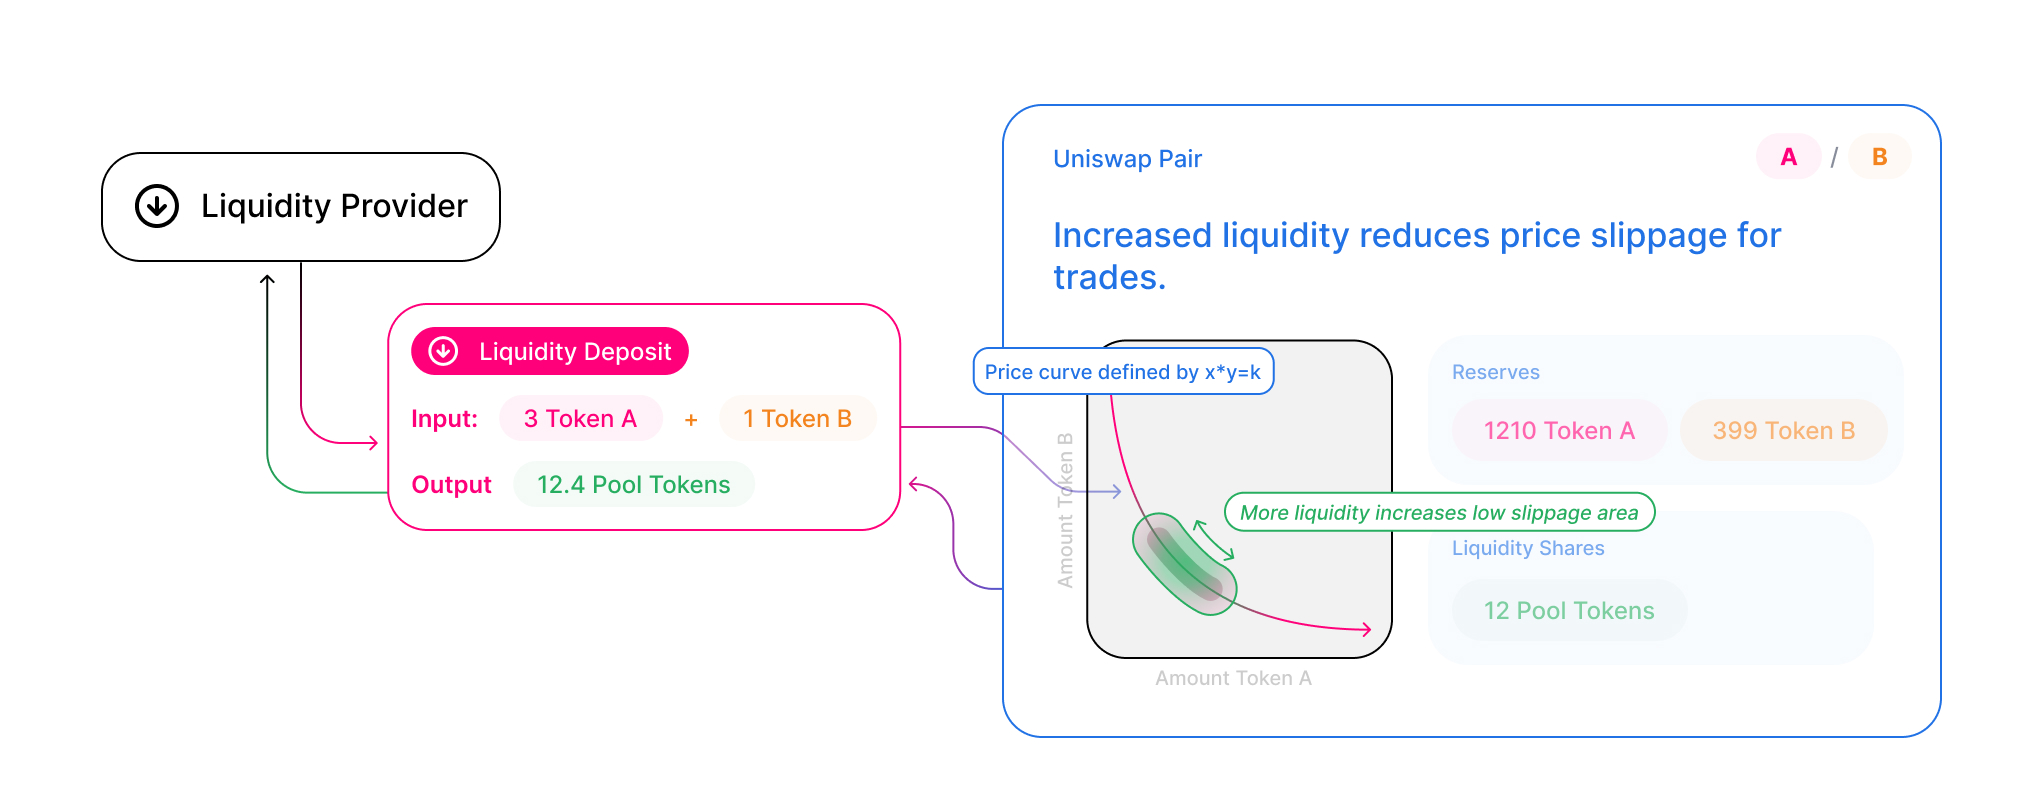
\includegraphics[width=\textwidth]{background/Images/uniswap_lp.jpeg}
    \caption{How Uniswap works~\cite{uniswap} \label{fig:uniswap_lp}}
\end{figure}

